\chapter{MIDI Setup}
\section{Connectivity:}

\begin{enumerate}
\item\textbf{Machinedrum}:
Connect the MIDI-Out of the Machinedrum to the MIDI-In (1) of the MegaCommand. and connect the MIDI-Out (1) of the MegaCommand to MIDI-In of the Machinedrum.

\item\textbf{External Midi:} (Optional): 
A MIDI Keyboard, or sequencer can be connected to MIDI-In (2). Attached MIDI Keyboards can be used to play notes in chromatic mode. Attached sequencers can be used as external clock source.

\item\textbf{Analog4:} (Optional):
Connect the MIDI-Out of the Analog4 to the MIDI-In (2) of the MegaCommand. and connect the MIDI-Out (2) of the MegaCommand to MIDI-In of the Analog 4.
\end{enumerate}
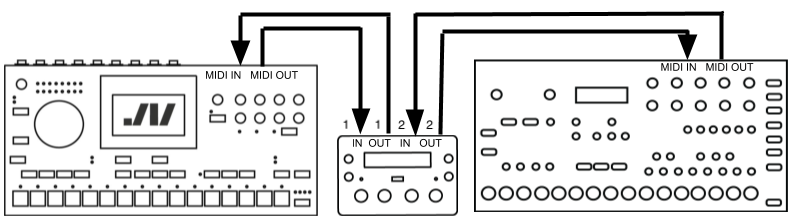
\includegraphics[scale=.6]{midi_machines.png}
\\
\section{MachineDrum Settings }

MCL communicates with the MachineDrum using SYSEX messages, and will configure your MD's global settings automatically. MCL will overwrite MD's global settings slots 7 and 8. These slots should always be reserved for MCL.

\section{Analog4 Settings:}

The following configuration must be manually applied in the Analog 4's Global Settings menu:

\begin{itemize}

\item{MIDI Port Config:}
\begin{enumerate}
\item{Output to MIDI}
\item{Input to MIDI}
\item{Keyboard CFG = EXT}
\item{Receive Notes = True}
\item{Receive CC/NPRN = True}
\end{enumerate}
\item{MIDI Channels:}

Tracks 1-6 channels need to be set to MIDI Channels 1-6 respectively.

\end{itemize}

\section{Turbo MIDI}

MCL supports Elektron's Turbo MIDI protocol with selectable speeds 1x, 2x, 4x, 8x.\\
\\
Each MIDI port can be configured with a unique speed and is configurable in the \textbf{MIDI Menu} accessible from \textbf{Global Settings}.
\\
\\
\textit{For optimal firmware performance, reduced transmission latency and lowest sequencer jitter, use the default \textbf{Turbo 8x speed.}}

\section{Active Peering:}

When a MIDI device is connected to ports 1 or 2. The MegaCommand will automatically detect the attached device and set the chosen Turbo MIDI speed. If the attached device cannot be identified it will default to General MIDI (GM) Device.\\
\\
\textit{MCL has no method of detecting a snapshot change on the MachineDrum. If a new snapshot is loaded on the MD either the MC or MD will need to be powercycled to reform the peer.}


 
